\begin{flushright} {\tiny {\color{gray} benchmark\_vaks97.tex}} \end{flushright}

\vspace{1cm}
\begin{flushright}
Data pertaining to this section are to be found at:
\url{https://github.com/cedrict/fieldstone/tree/master/images/benchmark_vaks97}
\end{flushright}
\vspace{1cm}


This numerical experiment was first presented in \textcite{vaks97} (1997).
It consists of an isothermal Rayleigh-Taylor instability in a two-dimensional box
of size $Lx=0.9142$ and $L_y=1$.

Two Newtonian fluids are present in the system: the buoyant layer is 
placed at the bottom of the box and the interface between both fluids 
is given by 
\begin{equation}
y(x)=0.2+0.02\cos \left( \frac{\pi x}{L_x}  \right)
\end{equation}
The bottom fluid is parametrised by its density $\rho_1=1000$ and 
its viscosity $\eta_1$, while the layer above is parametrised 
by $\rho_2=1010$ and $\eta_2=100$.
This experiment is to be carried out for various viscosity constrasts between the 
two layers, i.e. $\eta_1=\{1,10,100\}$.

No-slip boundary conditions are applied at the bottom and at the top of the box 
while free-slip boundary conditions are applied on the sides.
Gravity is pointing downwards with $|\vec{g}|=10$. 

\begin{center}
\includegraphics[width=4cm]{images/benchmark_vaks97/elefant256_0500.png}
\includegraphics[width=4cm]{images/benchmark_vaks97/elefant256_1000.png}
\includegraphics[width=4cm]{images/benchmark_vaks97/elefant256_1500.png}
\includegraphics[width=4cm]{images/benchmark_vaks97/elefant256_2000.png}\\
{\captionfont Example of time evolution obtained with the \elefant code for 
a 256x256 grid with the particle-in-cell method.\\
{\tiny {\color{gray} in images/benchmark\_vaks97/}}  }
\end{center}

One can measure the following quantities:

\begin{itemize}

\item the root mean square velocity $\upnu_{rms}$ in the domain as a function of time:
\begin{equation}
\upnu_{rms}= \sqrt{ \frac{1}{L_xL_y} \int \int |{\vec \upnu}|^2 dxdy}
\end{equation}

\item the maximum (or local maxima) of the $\upnu_{rms}$ and 
its (their) corresponding time(s)

\item the growth rate of the instability at $t=0$.
From linear stability analysis, the analytical growth rate can 
be calculated \cite{ramb68,ramb81}: 
$\gamma_{th}=0.01094019$, which is valid for an infinitesimal perturbation. 
For each model run, the growth rate $\gamma$ is measured by fitting 
the $\upnu_{rms}$ and/or (?) the maximum 
vertical velocity measurements for a short time $t$. 

\item the total mass of the system $M(t)$ as a function of time. 
Since there is no chemical diffusion in the 
system (pure advection equation) the amount of material in the system 
is to remain constant, and therefore its mass too.
\begin{equation}
M(t) = \int \int \rho(x,y,t) dxdy
\end{equation}
Given the layout described in the previous paragraph, the exact 
analytical initial mass $M_0$ of the system is given by 
\[
M_0=0.9142 \times (0.2 \times 1000 + 0.8\times 1010) = 921.5136
\]
The average density is then 
\[
<\rho>_0=\frac{M_0}{L_xL_y} = 1008
\]
We will then measure the relative mass error as a function of time
\[
\delta M(t) = \frac{M(t)-M_0}{M_0}
\]
which is equal to 
\[
<\delta\rho>(t) = \frac{<\rho>(t)-<\rho>_0}{<\rho>_0}
\]

\item the length of the interface between the fluids. At startup it is given by 
\[
{\cal L}(0) = \int_0^L \sqrt{1 + (dy/dx)^2} dx
\]
with $y(x)=0.2+0.02\cos(\pi x/L)$. Using WolframAlpha, we find
\[
{\cal L}(0)= \frac{L}{\pi} \int_0^\pi \sqrt{1 + 
\left(0.02\frac{\pi}{L}\sin(\pi x /L) \right)^2} dx
\simeq 0.9152786349
\]

\end{itemize}


\paragraph{Instantaneous results}.
Results obtained with \stone~\ref{f25} ($Q_2\times Q_1$ element) 
and \stone~\ref{f93} ($P_2^+\times P_{-1}$ element), 
both with mesh fitted so as to follow the interface between both fluids.

\begin{center}
\begin{tabular}{llp{4cm}p{4cm}p{4cm}}
\hline
            &  & $\eta_1=100$ &  $\eta_1=10$ &  $\eta_1=1$ \\ 
\hline\hline
$\min(u)$   & Stone 25 &  & & -4563.5\\
            & Stone 93 ($P_2^+\times P_{-1}$) &  & &        \\
            & Aspect   &  & &        \\
\hline
$\max(u)$   & Stone 25 &  &  & 1054.03\\
            & Stone 93 ($P_2^+\times P_{-1}$)&  & &        \\
            & Aspect   &  & &        \\
\hline
$\min(v)$   & Stone 25 &  &  & \\
            & Stone 93 ($P_2^+\times P_{-1}$)&  & &        \\
            & Aspect   &  & &        \\
\hline
$\max(v)$   & Stone 25 &  &  & 2070.9\\
            & Stone 93 ($P_2^+\times P_{-1}$)&  & &        \\
            & Aspect   &  & &        \\
\hline
$\max(|v|)$ & Stone 25 & 422.125 & & 4563.67\\
            & Stone 93 ($P_2^+\times P_{-1}$)&  & &        \\
            & Aspect   &  & &        \\
\hline
$v_{rms}$   & Stone 25 & 185.2947 & & 1441.87\\
            & Stone 93 ($P_2^+\times P_{-1}$)&  & &        \\
            & Aspect   &  & &        \\
\hline
$\min(p)$   & Stone 25 & -5048.16 & & -5048.7345\\ 
            & Stone 93 ($P_2^+\times P_{-1}$)&  & &        \\
            & Aspect   &  & &        \\
\hline
$\max(p)$   & Stone 25 & 5033.6947 & & 5032.329\\
            & Stone 93 ($P_2^+\times P_{-1}$)&  & &        \\
            & Aspect   &  & &        \\
\hline
\end{tabular}
\end{center}






\newpage



\begin{center}
\begin{tabular}{lllllll}
\hline
Code & Grid & Method & Growth Rate $\gamma$ & t (max vrms) & max (vrms)   & publication\\
\hline\hline
HS & 41x41 & extrapolated & 0.010996 & 211.1  & 0.0030958 & \cite{vaks97}\\
   & 61x64 & extrapolated & 0.011109 & 209.17 & 0.0031022 & \\
   & 81x81 & extrapolated & 0.011177 & 208.99 & 0.0030916 & \\
\hline
CND & 32x32 && 0.01106 & 208.4 & 0.003092 & \cite{vaks97}\\
    & 48x48 && 0.01106 & 208.5 & 0.0030943 \\
\hline 
SK &   80x80 && 0.01130 & 215.67 & 0.00299279 & \cite{vaks97}\\
   & 120x120 && 0.01127 & 206.38 & 0.0028922 \\
   & 160x160 && 0.01179 & 207.84 & 0.0028970 \\
\hline
PvK & 30x30 & splines & 0.01185 & 213.38 & 0.00300 & \cite{vaks97}\\
    & 50x50 & splines & 0.01198 & 211.81 & 0.003016 \\
    & 80x80 & splines & 0.01207 & 210.75 & 0.003050 \\
    & 100x100 & splines & 0.01211 &  & \\
    & 30x30 & C1 element & 0.01253 & 210.59 & 0.003100 \\
    & 80x80 & C1 element & 0.01225 & 207.05 & 0.003091 \\
\hline
ISMM & 160x160	& &0.00991 & 230.1 & 0.003093	 &\cite{soga01}\\
ISMM & 120x120	& &0.00998 & 226.1 & 0.003133	 &\\
MSOU & 160x160	& &0.00993 & 231.4 & 0.003085	 &\\
MSOU & 120x120	& &0.01020 & 227.6 & 0.003134	 &\\
FSOU & 160x160	& &0.01111 & 217.3 & 0.003118	 &\\
FSOU & 120x120	& &0.01159 & 213.1 & 0.003151	 &\\
\hline
&64x64 	 &5 	&0.01112 	&206.5 	&0.003041 & \cite{taki03} \\
&	 &15 	&0.01117 	&208.8 	&0.003098 & \\
&	 &40 	&0.01115 	&209.9 	&0.003110 & \\
&128x128 &5 	&0.01113 	&208.1 	&0.003079 & \\
&	 &15 	&0.01110 	&208.9 	&0.003097 & \\
&	 &40 	&0.01109 	&209.2 	&0.003102 & \\
\hline
& 120x132 & Level sets & 0.01252 & 211.2 & 0.00301 & \cite{sunh10} \\
\hline
& 67m res. &  & &   215.3  & 0.003106 & \cite{chtl13} \\
& 100m res. & & &   215.28 & 0.003101 & \\
\hline
LaCoDe 	& 1808 elts (10754 dofs)   &&0.01221 & 215& 0.003110 & \cite{demh19} \\
	& 7093 elts (2592 dofs)    &&0.01222 & 212& 0.003080 & \\
	& 17960 elts (107468 dofs) &&0.01222 & 211& 0.003075 & \\
\hline
\end{tabular}\\
{\captionfont Selected Quantities for the Isoviscous Rayleigh-Taylor problem.
HS: FDM, stream function formulation, particles.
PvK: FEM, stream function, marker-chain.\\
SK: FEM, ConMan code, compositional field. 
CND: spline method, stream function formulation, particles.
}
\end{center}


List of literature showcasing results of the van Keken \etal (1997) \cite{vaks97} setup:
\begin{itemize}
\item de Smet \etal (2000) \cite{devv00a}. No table of results, only figures:
\begin{center}
\includegraphics[width=12cm]{images/benchmark_vaks97/devv00a_1}\\
\includegraphics[width=6cm]{images/benchmark_vaks97/devv00a_2}
\includegraphics[width=6cm]{images/benchmark_vaks97/devv00a_3}
\end{center}

\item Soboutia \etal (2001) \cite{soga01}. Results reported in table above.
\begin{center}
\includegraphics[width=6cm]{images/benchmark_vaks97/soga01a}
\includegraphics[width=6cm]{images/benchmark_vaks97/soga01b}
\end{center}

\item Babeyko \etal (2002) \cite{bast02}. No table of results, only one figure:
\begin{center}
\includegraphics[width=7cm]{images/benchmark_vaks97/bast02_a}
\includegraphics[width=7cm]{images/benchmark_vaks97/bast02_b}
\end{center}

\item Tackley \& King (2003) \cite{taki03}. Performed with grid resolutions of 
64x64 or 128x128 and with either 5, 15, or 40 tracers per cell (on average). 
Results reported in table above. 

\begin{center}
\includegraphics[width=5.27cm]{images/benchmark_vaks97/taki03_a}
\includegraphics[width=5.27cm]{images/benchmark_vaks97/taki03_d}
\includegraphics[width=5.27cm]{images/benchmark_vaks97/taki03_e}
\end{center}

There are also results for non-isoviscous cases.

\item Bourgouin \etal (2006) \cite{bomh06}. No table of results, only figures.
Additional results for non-isoviscous in the paper.

\begin{center}
\includegraphics[width=7cm]{images/benchmark_vaks97/bomh06_a}
\includegraphics[width=7cm]{images/benchmark_vaks97/bomh06_b}
\end{center}

\item Quinteros \etal (2009) \cite{qurj09}.

\begin{center}
\includegraphics[width=5cm]{images/benchmark_vaks97/qurj09_a}
\includegraphics[width=5cm]{images/benchmark_vaks97/qurj09_b}
\includegraphics[width=5cm]{images/benchmark_vaks97/qurj09_c}
\end{center}

"Different snapshots from the domain evolution that are shown in Fig. 10 were compared with the 
ones published by van Keken \etal (1997). The evolution shown in this chapter and 
in the van Keken paper are identical for all the compared time steps."

\item Samuel \& Evonuk (2010) \cite{saev10}.

\begin{center}
\includegraphics[width=4cm]{images/benchmark_vaks97/saev10_a}
\includegraphics[width=5cm]{images/benchmark_vaks97/saev10_b}\\
\includegraphics[width=5cm]{images/benchmark_vaks97/saev10_c}
\includegraphics[width=5cm]{images/benchmark_vaks97/saev10_d}
\end{center}

\item Suckale \etal (2010) \cite{sunh10}.

\begin{center}
\includegraphics[height=7cm]{images/benchmark_vaks97/sunh10_a}
\includegraphics[height=7cm]{images/benchmark_vaks97/sunh10_e}\\
{\captionfont The Rayleigh-Taylor instability at t = 1500 computed by (left) 
the level set method on a 300x330 grid, compared to the best results\\ 
of (right) the four codes compared by van Keken \etal }\\
b)\includegraphics[width=4.5cm]{images/benchmark_vaks97/sunh10_b}
c)\includegraphics[width=5cm]{images/benchmark_vaks97/sunh10_c}
d)\includegraphics[width=5.2cm]{images/benchmark_vaks97/sunh10_d}\\
{\captionfont 
b) Detailed comparison of the level set (thin black line) and the marker chain 
approach (thick grey line) for the isothermal and isoviscous Rayleigh-Taylor 
instability at nondimensional time t = 1500. The plotted interfaces represent a 
zoom onto the instability descending from the top downwards in the middle of the box. 
The two methods yield an almost identical interface. 
c) Evolution of the entrainment of the buoyant fluid over time as computed by 
the five different codes. The level set computation was done on a 160$\times$176 grid.
d) Evolution of the root mean square velocity of the interface over time 
as computed by the five different codes. The level set computation was done on a 160$\times$176 grid.}
\end{center}

\begin{center}
a)\includegraphics[width=6cm]{images/benchmark_vaks97/sunh10_f}
b)\includegraphics[width=6cm]{images/benchmark_vaks97/sunh10_g}\\
{\captionfont Taken from the supplementary material: a) Convergence test for the isothermal and isoviscous Rayleigh-Taylor instability, benchmark problem 3.
A lack of convergence is easiest to identify during the phases of rapid rise of an instability. We illustrate this for the rise of
the secondary instability on the right side of the box at time t=1000 and four different grid sizes: 60x66, 80x88, 100x110,
and 120x132. We observe convergence for grid sizes above 100x110.\\
b) Convergence test for the isothermal and isoviscous Rayleigh-Taylor instability, benchmark problem 3.
We illustrate this convergence test for the rise of the secondary instability at time $t=1000$. The four
interfaces were computed based on the time steps: $\Delta t = 180 \Delta x$, $\Delta t = 90 \Delta x$, 
$\Delta t = 45 \Delta x$, and $\Delta t = 25 \Delta x$. We observe convergence for time steps $\Delta t \le 25 \Delta x$.
}
\end{center}

\begin{center}
a) \includegraphics[height=5cm]{images/benchmark_vaks97/sunh10_h}
b) \includegraphics[height=5cm]{images/benchmark_vaks97/sunh10_i}\\
{\captionfont 
a) The isothermal Rayleigh-Taylor instability with viscosity contrast 10 at non-dimensional time
t=500. The computation was done with a grid resolution of 250$\times$275. 
b) The Rayleigh-Taylor instability as computed by the HS-tracer method at time t=1500. The equations
of motion for this simulation were solved on an 81$\times$81 grid. The right panel is a zoom onto the peak located left of the
descending instability. Each blue dot represents one particle and the grid represents a rough estimate of the scale at which
the flow field is approximated correctly.
}
\end{center}


\item Leng \& Zhong (2011) \cite{lezh11}.

\begin{center}
\includegraphics[width=6cm]{images/benchmark_vaks97/lezh11_a}
\includegraphics[width=9cm]{images/benchmark_vaks97/lezh11_b}\\
{\captionfont Left: The mesh distribution and chemical composition for case RT1 at 
two different times: (a and c) t = 0 and (b and d) t = 1500. 
Right: a) The root mean square velocity $\upnu_{rms}$ and (b) the relative entrainment of 
the buoyant material, with time for case RT1. The corresponding benchmark results from 
van Keken \etal [1997] are also plotted.} 
\end{center}


\item Vynnytska \etal (2013) \cite{vyrc13}. Results only for 100 viscosity contrast


\item Choi \etal (2013) \cite{chtl13}.

\begin{center}
\includegraphics[width=7cm]{images/benchmark_vaks97/chtl13_a}
\includegraphics[width=7cm]{images/benchmark_vaks97/chtl13_b}\\
{\captionfont 
Left:
Rayleigh-Taylor instability. (a) Model setup. Snapshots of the density at dimensionless 
time of (b) 500, (c) 1000, and (d) 1500. (e) Plot of $\upnu_{rms}$ versus dimensionless time, t. 
The resolution is about $0.6\si{\kilo\metre}$. 
Right:
$\sigma_{xx}$ and density fields before and after the first remeshing with about $1\si{\kilo\metre}$ 
resolution. 
The white lines in the ``After'' images denote the original phase boundary before remeshing. 
The thick-lined box in the inset shows the location of the zoomed-in part of the domain.}
\end{center}


\item Fuchs \& Schmeling (2013) \cite{fusc13}.

\begin{minipage}{.99\linewidth}
\begin{center}
\includegraphics[width=7cm]{images/benchmark_vaks97/fusc13}\\
{\captionfont 
Finite deformation field for different stages of the diapirism with three 
different viscosity ratios and an initial non-dimensional thickness of 
the buoyant layer $h_2=0.2$. 
Left column: viscosity ratio $m = 0.1$. 
Middle column: $m = 1$. 
Right column: $m = 10$. 
Top row: pillow stage. 
Middle row: rising stage. 
Lower row: final stage. }
\end{center}
\end{minipage}


\item de Montserrat \etal (2019) \cite{demh19}.


\begin{center}
\includegraphics[width=7cm]{images/benchmark_vaks97/demh19}\\
{\captionfont 
a-e) Temporal evolution of the Rayleigh-Taylor instability. 
f) Evolution of $\upnu_{rms}$. 
Remeshing of the domain is necessary when the mesh becomes highly distorted. 
Note that the red lines overlap with the blue line. 
g) Second invariant of the accumulated strain in a mesh with heavily distorted elements, 
and h) interpolated into a new high-quality mesh. 
i) Histogram showing the logarithm of the error between the accumulated square root of 
second invariant of the strain rate, pre- and post-remeshing.}
\end{center}


\item Robey \& Puckett (2019) \cite{ropu19}, Robey (2019) \cite{robe19} (PhD thesis).

\begin{center}
\includegraphics[width=5cm]{images/benchmark_vaks97/ropu19}\\
{\captionfont Computed solution of the van Keken isoviscous Rayleigh-Taylor problem
at time $t = 2000$ on a uniform grid of 128x128 cells. }
\end{center}



\item Louis-Napoleon \etal (2020) \cite{logb20}.

Raw data available in {\tt ./images/benchmark\_vaks97/louis\_napoleon\_etal}.

\begin{center}
\includegraphics[width=11cm]{images/benchmark_vaks97/louis_napoleon_etal/VK1}\\
\includegraphics[width=14cm]{images/benchmark_vaks97/louis_napoleon_etal/VKzoom}
\end{center}

\item Maierova (2012) \cite{maie12} (phd thesis)

\begin{center}
\includegraphics[width=8cm]{images/benchmark_vaks97/maie12_b}
\includegraphics[width=11cm]{images/benchmark_vaks97/maie12_a}\\
{\captionfont Time 500,1000, 2000.}
\end{center}


\item Schuh-Senlis \etal (2020) \cite{sctc20}. The setup in the paper is inspired 
by \cite{vaks97} but results are therefore not consistent with those of \cite{vaks97}.

\begin{center}
\includegraphics[width=4cm]{images/benchmark_vaks97/schuh_senlis_etal/fig04}
\includegraphics[width=7cm]{images/benchmark_vaks97/schuh_senlis_etal/fig05}
\end{center}

\item MVEP2 code, curtesy of Marcel Thielmann \index{contributors}{M. Thielmann}

\begin{center}
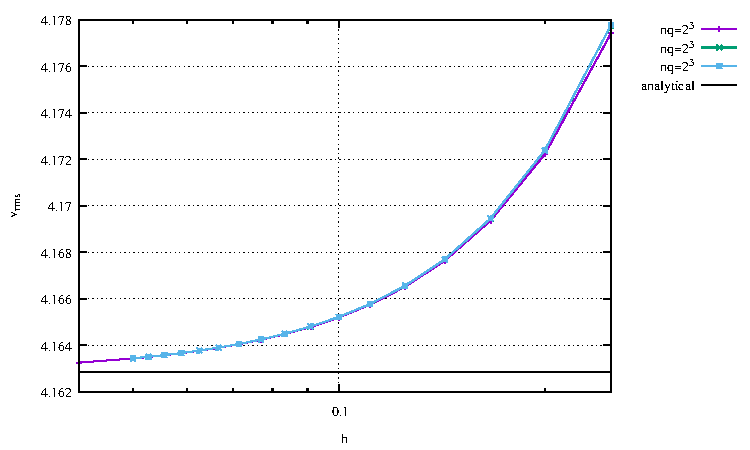
\includegraphics[width=7cm]{images/benchmark_vaks97/MVEP2/vrms.pdf}
\end{center}

\item \textcite{buoa24} (2024).

\begin{center}
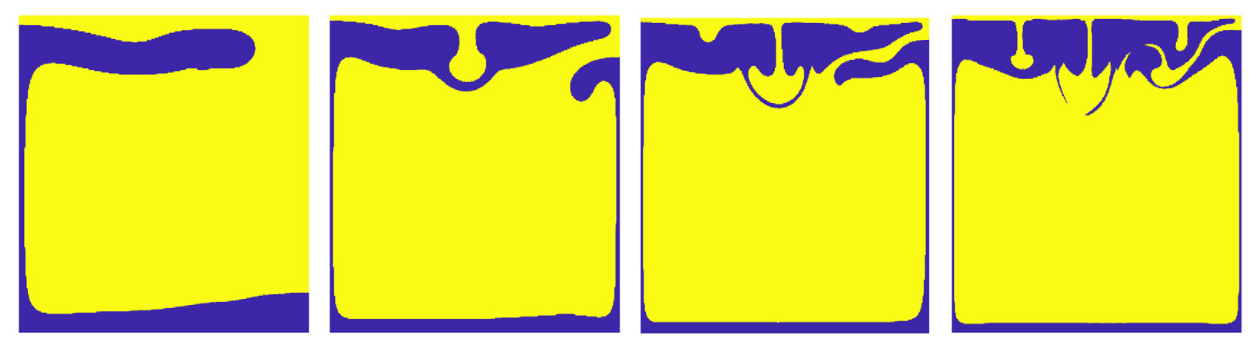
\includegraphics[width=12cm]{images/benchmark_vaks97/buoa24/buoa24_1}\\
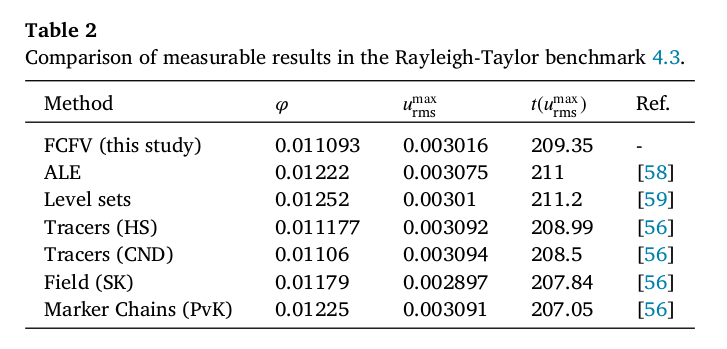
\includegraphics[width=7cm]{images/benchmark_vaks97/buoa24/buoa24_2}
\end{center}




\item Logg \etal (2012) \cite{lomw12}: only Entrainment of a Dense Layer by Thermal convection.

\newpage
\item \aspect{} manual \cite{aspectmanual}.

\begin{center}
\includegraphics[width=3cm]{images/benchmark_vaks97/aspect/lvl7/composition0000}
\includegraphics[width=3cm]{images/benchmark_vaks97/aspect/lvl7/composition0001}
\includegraphics[width=3cm]{images/benchmark_vaks97/aspect/lvl7/composition0002}
\includegraphics[width=3cm]{images/benchmark_vaks97/aspect/lvl7/composition0003}
\includegraphics[width=3cm]{images/benchmark_vaks97/aspect/lvl7/composition0004}\\
\includegraphics[width=3cm]{images/benchmark_vaks97/aspect/lvl7/composition0005}
\includegraphics[width=3cm]{images/benchmark_vaks97/aspect/lvl7/composition0006}
\includegraphics[width=3cm]{images/benchmark_vaks97/aspect/lvl7/composition0007}
\includegraphics[width=3cm]{images/benchmark_vaks97/aspect/lvl7/composition0008}
\includegraphics[width=3cm]{images/benchmark_vaks97/aspect/lvl7/composition0009}\\
\includegraphics[width=3cm]{images/benchmark_vaks97/aspect/lvl7/composition0010}
\includegraphics[width=3cm]{images/benchmark_vaks97/aspect/lvl7/composition0011}
\includegraphics[width=3cm]{images/benchmark_vaks97/aspect/lvl7/composition0012}
\includegraphics[width=3cm]{images/benchmark_vaks97/aspect/lvl7/composition0013}
\includegraphics[width=3cm]{images/benchmark_vaks97/aspect/lvl7/composition0014}\\
\includegraphics[width=3cm]{images/benchmark_vaks97/aspect/lvl7/composition0015}
\includegraphics[width=3cm]{images/benchmark_vaks97/aspect/lvl7/composition0016}
\includegraphics[width=3cm]{images/benchmark_vaks97/aspect/lvl7/composition0017}
\includegraphics[width=3cm]{images/benchmark_vaks97/aspect/lvl7/composition0018}
\includegraphics[width=3cm]{images/benchmark_vaks97/aspect/lvl7/composition0019}\\
---------------------------------------\\
\includegraphics[width=3cm]{images/benchmark_vaks97/aspect/lvl7/composition_threshold0000}
\includegraphics[width=3cm]{images/benchmark_vaks97/aspect/lvl7/composition_threshold0001}
\includegraphics[width=3cm]{images/benchmark_vaks97/aspect/lvl7/composition_threshold0002}
\includegraphics[width=3cm]{images/benchmark_vaks97/aspect/lvl7/composition_threshold0003}
\includegraphics[width=3cm]{images/benchmark_vaks97/aspect/lvl7/composition_threshold0004}\\
\includegraphics[width=3cm]{images/benchmark_vaks97/aspect/lvl7/composition_threshold0005}
\includegraphics[width=3cm]{images/benchmark_vaks97/aspect/lvl7/composition_threshold0006}
\includegraphics[width=3cm]{images/benchmark_vaks97/aspect/lvl7/composition_threshold0007}
\includegraphics[width=3cm]{images/benchmark_vaks97/aspect/lvl7/composition_threshold0008}
\includegraphics[width=3cm]{images/benchmark_vaks97/aspect/lvl7/composition_threshold0009}\\
\includegraphics[width=3cm]{images/benchmark_vaks97/aspect/lvl7/composition_threshold0010}
\includegraphics[width=3cm]{images/benchmark_vaks97/aspect/lvl7/composition_threshold0011}
\includegraphics[width=3cm]{images/benchmark_vaks97/aspect/lvl7/composition_threshold0012}
\includegraphics[width=3cm]{images/benchmark_vaks97/aspect/lvl7/composition_threshold0013}
\includegraphics[width=3cm]{images/benchmark_vaks97/aspect/lvl7/composition_threshold0014}\\
\includegraphics[width=3cm]{images/benchmark_vaks97/aspect/lvl7/composition_threshold0015}
\includegraphics[width=3cm]{images/benchmark_vaks97/aspect/lvl7/composition_threshold0016}
\includegraphics[width=3cm]{images/benchmark_vaks97/aspect/lvl7/composition_threshold0017}
\includegraphics[width=3cm]{images/benchmark_vaks97/aspect/lvl7/composition_threshold0018}
\includegraphics[width=3cm]{images/benchmark_vaks97/aspect/lvl7/composition_threshold0019}\\
{\captionfont Time evolution of the system, smooth compositional field, CFL=0.25, 
mesh refinement level 8. Top block is with 256 colors, bottom block is the same data 
but only using two colors. From t=0 until t=2000, every 100s.}
\end{center}

When compositional fields are used the solution has been shown (see \aspect manual)
to be very sensitive to the resolution. In an attempt to remedy this issue, 
an approach was devised, which consists in replacing the original discontinuous initial 
condition with a smoothed out version. The function in the input file 
\begin{lstlisting}
set Function expression = if( (z>0.2+0.02*cos(pi*x/0.9142)) , 0 , 1 )
\end{lstlisting}
is then replaced by 
\begin{lstlisting}
set Function expression = 0.5*(1+tanh((0.2+0.02*cos(pi*x/0.9142)-z)/0.02))
\end{lstlisting}
The last number on the line is a parameter which controls the 'thickness' of the interface.
When it becomes small we recover a discontinuous implementation (this very much 
depends on the mesh size). 


\begin{center}
\includegraphics[width=5.4cm]{images/benchmark_vaks97/aspect/velocity-discontinuous}
\includegraphics[width=5.4cm]{images/benchmark_vaks97/aspect/velocity-smooth}
\includegraphics[width=5.4cm]{images/benchmark_vaks97/aspect/smoothing-parameter-velocity}\\
{\captionfont Taken from the \aspect manual. 
Root mean square measurements with discontinuous (left) and smoothed, continuous 
(middle) initial conditions for the compositional field: 5 global refinements correspond to 
a $32\times 32$ mesh, 9 refinements to a $512 \times 512$ mesh.
Right: influence of smoothing parameter (level 7).}
\end{center}


\begin{minipage}{.99\linewidth}
\begin{center}
\includegraphics[width=5.4cm]{images/benchmark_vaks97/vrms6}
\includegraphics[width=5.4cm]{images/benchmark_vaks97/vrms7}
\includegraphics[width=5.4cm]{images/benchmark_vaks97/vrms8}\\
\includegraphics[width=5.4cm]{images/benchmark_vaks97/vrms6_peak1}
\includegraphics[width=5.4cm]{images/benchmark_vaks97/vrms7_peak1}
\includegraphics[width=5.4cm]{images/benchmark_vaks97/vrms8_peak1}\\
\includegraphics[width=5.4cm]{images/benchmark_vaks97/vrms6_peak2}
\includegraphics[width=5.4cm]{images/benchmark_vaks97/vrms7_peak2}
\includegraphics[width=5.4cm]{images/benchmark_vaks97/vrms8_peak2}\\
\includegraphics[width=5.4cm]{images/benchmark_vaks97/C1_6}
\includegraphics[width=5.4cm]{images/benchmark_vaks97/C1_7}
\includegraphics[width=5.4cm]{images/benchmark_vaks97/C1_8}\\
{\captionfont Results obtained for both approaches and vof, on various meshes and for 
various smoothing parameters. The dashed lines indicate the \stone 95 results.}
\end{center}
\end{minipage}


\begin{center}
\includegraphics[width=10cm]{images/benchmark_vaks97/aspect/C1}\\
{\captionfont Results for smoothed approach. Left to right: level 6,7,8. Top to bottom: smoothing 
parameter 0.0025, 0.005, 0.01, 0.02. We see that level6 results in combination with a small smoothing parameter
yield a very different outcome.}
\end{center}

\begin{center}
\includegraphics[height=6cm]{images/benchmark_vaks97/aspect/contours_678}
\includegraphics[height=6cm]{images/benchmark_vaks97/aspect/contours_678zoom}\\
{\captionfont 0.5 compositional field $C_1$ isocontours for all 12 simulations.} 
\end{center}

\begin{center}
\includegraphics[height=5cm]{images/benchmark_vaks97/aspect/contours_78}
\includegraphics[height=5cm]{images/benchmark_vaks97/aspect/contours_8}\\
{\captionfont 0.5 compositional field $C_1$ isocontours for levels 7 and 8 (left), 
and level 8 (right)} 
\end{center}


\newpage
The code can also rely on the VOF method to solve the advection equation 
for the computational fields:

\begin{center}
\includegraphics[width=9cm]{images/benchmark_vaks97/aspect_vof/rms_vel_comparison.png}
\includegraphics[width=6cm]{images/benchmark_vaks97/aspect_vof/vof_van_keken_refinement_comparison.png}\\
{\captionfont 
Left:
Evolution of the root mean square velocity as a function of time for computations 
of the van Keken problem made with the VOF interface tracking algorithm with five 
different global mesh refinements (from a $32 \times 32$ mesh 
to a $1024 \times 1024$ mesh.
Right:
The results of two computations of the van Keken problem made with the VOF 
interface tracking algorithm overlaid upon each other at $t_\text{end}=2000$.
This visualization shows the reconstructed boundary between the two
materials at the final time $t_\text{end}$ as computed on a uniform grid
with 7 and 8 levels of refinement.
The boundaries between the materials are displayed as contours
of the fields $\tilde{\psi}^7(t_\text{end})$ (black) and
$\tilde{\psi}^8\,(t_\text{end})$ (bright green), which are generated by the  visualization postprocessor.
The contours for the reconstructed material boundaries are superimposed
on a color gradient visualization of the material composition for the
computation with 8 levels of refinement in order to make the regions
with each fluid type more evident.   }
\end{center}

\item Mulyokova phd thesis \cite{mulyukova} 

\begin{center}
\includegraphics[width=8cm]{images/benchmark_vaks97/mulyukova1}
\includegraphics[width=8cm]{images/benchmark_vaks97/mulyukova2}
\end{center}


\end{itemize}

\begin{landscape} 
\begin{scriptsize}
\begin{tabular}{l|lllllllllll|l}
\hline
Publication & $\eta^\star$ & Stokes  & Transport  
& vrms & png & max & peak 1 & peak 1 & peak 2 & peak 2  & growth rate &  observation \\
&& method & method & && time & time & vrms & time & vrms & rate & \\
\hline\hline
van Keken \etal \cite{vaks97} 
&1&&& $\surd$ & $\surd$ & 2000 & 211.1 & 0.0030958&     &    & 0.010996 & HS 41x41 \\
&1&&&&&& 209.17&0.0031022  && & 0.011109 & HS 61x61  \\
&1&&&&&& 208.99&0.0030916  && & 0.011177 & HS 81x81  \\
&1&&&&&& 208.4 &0.003092   && & 0.01106  & CND 32x32  \\
&1&&&&&& 208.5 &0.0030943  && & 0.01106  & CND 48x48  \\
&1&&&&&& 215.67&0.00299279 && & 0.01130  & SK 80x80  \\
&1&&&&&& 206.38&0.0028922  && & 0.01127  & SK 120x120  \\
&1&&&&&& 207.84&0.0028970  && & 0.01179  & SK 160x160  \\
&1&&&&&&       &           && & 0.01220  & SK 160x160  \\
&1&&&&&& 213.38&0.00300    && & 0.01185  & PvK 30x30 splines   \\
&1&&&&&& 211.81&0.003016   && & 0.01198  & PvK 50x50 splines   \\
&1&&&&&& 210.75&0.003050   && & 0.01207  & PvK 80x80 splines   \\
&1&&&&&&       &           && & 0.01211  & PvK 100x100 splines   \\
&1&&&&&& 210.59&0.003100   && & 0.01253  & PvK 30x30 C1   \\
&1&&&&&& 207.05&0.003091   && & 0.01225  & PvK 80x80 C1   \\ \hline
de Smet \etal \cite{devv00a} & \\ \\ \hline
Sobouti \etal \cite{soga01} & \\ \\ \hline
Babeyko \etal \cite{bast02} & \\ \\ \hline
Tackley \& King \cite{taki03} & \\ \\ \hline
Bourgouin \etal \cite{bomh06} & \\ \\ \hline
Quinteros \etal \cite{qurj09} & \\ \\ \hline
Samuel \& Evonuk \cite{saev10} & \\ \\ \hline
Suckale \etal \cite{sunh10} & 1  & FDM &level set & $\surd$ & $\surd$ & 1500 & 211.2  &0.00301 & ? & ? & 0.01252  & 120x132  \\ \hline
Suckale \etal \cite{sunh10} & 10 & FDM &level set & $\surd$ & $\surd$ &  500 & ?      & ?      & ? & ? & 0.04809  & 250x275  \\ \hline
Leng \& Zhong \cite{lezh11} & 1  & FEM & tracers  & $\surd$ & $\surd$ & 1500 & ?      & ?      & ? & ? & ?        & AMR(6+3) \\ \hline
Maierova PhD thesis \cite{maie12}  
&   1 &&&Y& Y &2000 &211 & 0.003107\\ 
& 0.1 &&&Y& N &2000 &73 & 0.009411 \\ 
& 100 &&&Y& N &2000 &51 & 0.013938 \\ 
\\ \hline
Vynnytska \etal \cite{vyrc13} & \\ \\ \hline
Choi \etal \cite{chtl13} & \\ \\ \hline
Fuchs \& Schmeling \cite{fusc13} & \\ \\ \hline
Mulyukova PhD thesis\cite{mulyukova}  & \\ \\ \hline
de Montserrat \etal \cite{demh19} & \\ \\ \hline
Robey \& Puckett \cite{ropu19} & \\ \\ \hline
Robey PhD thesis \cite{robe19}  & \\ \\ \hline
Trim \etal (2021) \cite{trbs21} & \\ \\ \hline
Louis-Napoleon \etal \cite{logb20} & 1 & FEM & VOF \& CF& &&&&&&&& JADIM, OpenFOAM \& \aspect{}   \\ \\
\hline
\aspect{} manual \cite{aspectmanual} & 1  & FEM & CF, PIC & $\surd$ 
& $\surd$ &  \\ \\
\hline
\end{tabular}
\end{scriptsize}
\end{landscape}

